% !TEX root = emsoft-2019.tex
%\vspace{-0.4cm}
\section{Aggregation and Deaggregation}
\label{sec:agdag}
%\vspace{-0.2cm}

In aggregation, the set of all stars in $queueStars$ that are making a discrete transition to the same mode are collected together. 
%
Say, these states are $S_1, S_2, \ldots, S_m$.
%
Then, an overapproximation of these $S'$ is computed such that $S_1 \cup S_2 \cup S_3 \ldots \cup S_m \subseteq S_{over}$. 
%
Instead of computing the reachable set for each of $S_1, S_2, \ldots, S_m$, the reachable set of $S_{over}$ is computed in the future modes.

There are two main drawbacks of this aggregation mechanism. 
%
First, the union of sets $S_1, S_2, \ldots, S_m$ is often a non-convex set. 
%
Whereas the representation used for computing reachable set is used for representing convex sets. 
%
Therefore, this overapproximation of a non-convex set by a convex set is very conservative.
%
More worryingly, the reachable set of $S_{over}$ will trigger additional discrete transitions that would not happen while computing the reachable sets using $S_1, S_2, \ldots, S_m$.
%
Such discrete transitions are artifacts of the conservative overapproximation during the aggregation process.


To overcome the two main challenges, we make the following modifications to the reachable set computation algorithm.
% to perform aggregation and deaggregation. 
%develop new aggregation and deaggregation techniques. Our technique works the following way. 
First, while handling discrete transitions, we perform aggregation for all the sets in the $queueStars$ that go to the same mode. 
%
The resultant star is tagged as an \textsf{aggregate} and the reachable set computation continues where the sets are tagged as \textsf{aggregate}. 
%
This way of computing the reachable set will result in a conservative overapproximation.
%
If one of the sets in the computation overlaps with the unsafe set $U$, we check if the set is tagged as \textsf{aggregate}.
%
If so, then we go to the initial set in the location and perform deaggregation and recompute the reachable set.
%
Hence, we perform counterexample guided deaggregation.
%
Our algorithm terminates after we find either a counterexample for safety specification or prove that the overapproximation of the reachable set does not overlap with unsafe set. 
%
The pseudocode description is given in Algorithm~\ref{alg:aggdeagg}.
%
A working example of the aggregation and deaggregation is provided in Figure~\ref{fig:deagg}.


\begin{algorithm}[h!]
\SetKwInOut{Input}{Input}\SetKwInOut{Output}{Output}\SetKw{Return}{return}
\SetAlgoVlined
\Input{Initial set $\Theta$, Hybrid automaton $H$, Step $h$, Bound $k$, Unsafe set $U$.}
\Output{If there exists a trajectory from $\Theta$ visits $U$.}
${\it queueStars} \gets \emptyset$\; 
append $(\Theta, loc_0, 0)$ to ${\it queueStars}$\; 
${\it ReachSet} \gets \emptyset$\;
\While{${\it queueStars}$ is not empty}{ \label{ln:begLoop}
    $S_1 \gets deque(queueStars)$\;
    \eIf{$S_1.tag = {\bf \sf unaggregated}$}{
        $S_{nxt} \gets S_1$\;
%        dequeue $S_1$ from $queueStars$
    }
    {
        $listAgg \gets$ stars in ${\it queueStars}$ with mode $S_1.loc$\; \label{ln:collectAggregate}
        $S_{nxt} \gets {\sf Aggregate}(listAgg)$\; \label{ln:aggregation}
%    stars in ${\it queueStars}$ going to same mode$)$\;
        $S_{nxt}.tag \gets {\bf \sf aggregated}$\; 
        dequeue $listAgg$ from $queueStars$\;   
    }
    $R \gets {\sf ReachSetDynamicalSystem}(S_{nxt}, S_{nxt}.loc)$\;
    $R' \gets {\sf InvariantOverlap}(R, R.loc)$\;
    \If{$R' \cap U \neq \emptyset$ and $R'.tag = {\sf aggregated}$ }{ \label{ln:deagg}
        $S_{agg} \gets$ first aggregated star in path from $S_{nxt}$ to $\Theta$\;
        $newStars \gets deaggregate(S_{agg})$\; 
        $newStars.tag \gets {\bf \sf unaggregated}$\;
%        Deaggregate at least one star in the path from $S_{agg}$ to root\;
        Enqueue $newStars$ into $queueStars$\;
    }
    \If{$R' \cap U \neq \emptyset$ and $R'.tag \neq {\sf aggregate}$}{ \label{ln:crucial}
        {\bf return} There exists a trajectory from $\Theta$ visiting $U$\;
    }
    ${\it ReachSet} \gets {\it ReachSet} \cup R'$\;
    ${\it nextRegions} \gets {\sf discreteTrans}(R', H.Trans)$\; \label{ln:guardIntersection}
    append ${\it nextRegions}$ to ${\it queueStars}$\; \label{ln:appendQueueStars}\label{ln:endLoop}
}
{\bf return} All trajectories are safe\;
\caption{Algorithm that performs aggregation and deaggregation for checking safety of the trajectories originating from $\Theta$.}
\label{alg:aggdeagg}
\end{algorithm}
%\vspace{-0.3cm}

In Algorithm~\ref{alg:aggdeagg}, the main loop (from lines~\ref{ln:begLoop}-~\ref{ln:endLoop}) continues until $queueStars$ is empty. 
%
We first dequeue a star from this queue and based on the tag, perform aggregation operation with all the stars for the same mode. 
%
We then compute the reachable set of the aggregated star in this mode. If one of the stars in the reachable set overlaps with the unsafe set, we check if the reachable set is tagged as $aggregated$. 
%
If so, we pick the first aggregated star in the path from the root $\Theta$ to the current star and perform deaggregation of the selected star.

These deaggregated stars are added to $queueStars$ with tag $unaggregated$ and the reachable set computation continues. 
%
If the reachable set of an $unaggregated$ star overlaps with the unsafe set, then the algorithm returns that the safety specification is violated.

%\vspace{-0.7cm}
\begin{figure}[h!]
\centerline{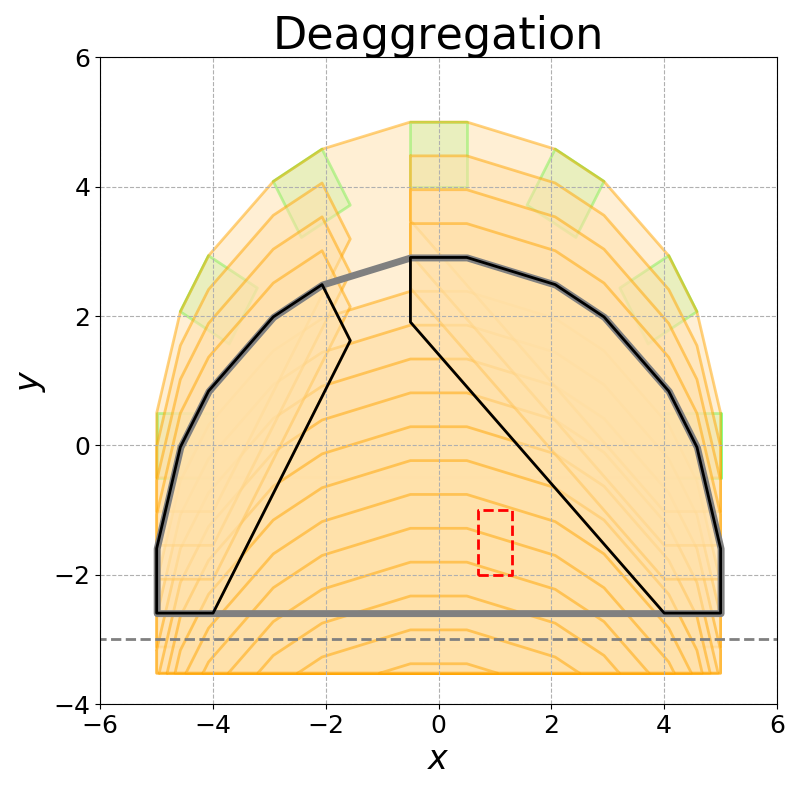
\includegraphics[width=0.7\columnwidth]{images/deagg.png}}
%\vspace{-0.4cm}
\caption{{\footnotesize The deaggregation process is shown for a two-mode system. Upon reaching an error mode (red dotted region), the fully aggregated set of states (gray large region), is split in half (two black regions), which no longer contain error states. A video of the complete computation is available online at \url{https://youtu.be/SDzGKDBq5tM}.}}
\label{fig:deagg}
\end{figure}
%\vspace{-0.7cm}


\begin{lemma}
Algorithm~\ref{alg:aggdeagg} will return safe if and only if all the simulations starting from $\Theta$ for bounded time $k$ are safe.
\end{lemma}
\begin{proof}
This proof is a consequence of simulation equivalent reachability of Algorithm~\ref{alg:algoHybrid}. 
%
We first prove that the Algorithm~\ref{alg:aggdeagg} is sound, that is, if the algorithm returns safe, then all simulations are indeed safe and if the algorithm returns unsafe, then it is indeed unsafe. 
%
If the condition in line~\ref{ln:crucial} of Algorithm~\ref{alg:aggdeagg} is satisfied, then the reachable set $R'$ is equivalent to the one computed without any aggregation and hence is simulation equivalent. 
%
Therefore the system is indeed unsafe. 
%
Hence, whenever the algorithm returns unsafe, the system is indeed unsafe. 
%
If the algorithm returns safe, then the reachable set computed using aggregation, which is clearly an overapproximation of the reachable set, does not overlap with unsafe set. 
%
Hence, the system is safe. 


It now remains to prove that the loop in lines~\ref{ln:begLoop}-~\ref{ln:endLoop} terminates after finite number of times. 
%
This is easy to infer as there are only finitely many reachable sets that we compute. 
%
Hence, we perform only finitely many aggregations. 
%
Since we strictly do not aggregate the stars that were deaggregated before, the condition in line~\ref{ln:deagg} will only be encountered finite number of times. 
%
Hence the loop terminates and the algorithm either returns safe or unsafe.
\end{proof}


One of the advantages of generalized stars is that it allows for easy aggregation and deaggregation. 
%In the remainder of this section, we demonstrate the advantages of performing aggregation 
%
Additionally, we avoid computing the entire reachable set, but only compute the specific sections of the reachable set that are important for safety verification.
%
To keep track of the aggregations and deaggregations, we maintain a data structure called Aggregated Directed Acyclic Graph (AGGDAG).
%
%The algorithm corresponding to the aggregation and deaggregation is given in Algorithm~\ref{alg:aggdeagg}. 
%%
%A working example of the aggregation and deaggregation is provided in Figure~\ref{fig:deagg}.




%\vspace{-0.3cm}
\subsection{Aggregation of Generalized Stars}
\label{sec:aggStars}
%\vspace{-0.1cm}

In this section, we present two techniques for performing aggregation of generalized stars. The first is template based aggregation and deaggregation and the second is aggregation using convex hulls.
% advantages of using generalized stars in aggregation and deaggregation. 
%


\subsubsection{Template Based Aggregation:}
\label{sec:templateAgg}
In this paper, since all the stars we encounter have predicates that are conjunctions of linear constraints, our overapproximation is also a predicate which is a conjunction of linear constraints.

\begin{lemma}
\label{lem:agg}
Consider stars $S_1 \deq \tup{a, G, P_1}$, $S_2 \deq \tup{a, G, P_2}$, $\ldots$, $S_m \deq \tup{a, G, P_m}$ where the anchor and generators for all the stars is the same.
%
A star $S' \deq \tup{a, G, P'}$ is an overapproximation of the union, i.e., $S_1 \cup S_2 \cup \ldots \cup S_m \subseteq S'$, if and only if $(P_1 \vee P_2 \vee \ldots \vee P_k) \Rightarrow P'$.
\end{lemma}
%\begin{proof}
%Trivially follows from the definition of generalized stars.
%\end{proof}

 For computing the predicate $P'$, we use a template based method.
%
% To compute the predicate $P'$, we perform a template based method. 
%
For each location, a set of template directions $c_1^{T}, c_2^{T}, \ldots, c_{l}^{T}$ are provided by the user and the predicate $P'$ is determined by selecting the appropriate values of $d_1, d_2, \ldots, d_l$ such that the condition $(P_1 \vee P_2 \vee \ldots \vee P_k) \Rightarrow P'$ is satisfied where $P' \deq (c_1^{T}\alpha \leq d_1) \wedge (c_2^{T}\alpha \leq d_2) \wedge \ldots \wedge (c_l^{T}\alpha \leq d_l)$. 

For computing $d_j$, $1 \leq j \leq l$, we solve $m$ linear programming problems. $d_j^i$ is the maximum value of $c_j^T \alpha$ in $P_i$. That is, $d_j^1 = \mathsf{max}~ c_j^T \alpha~ \mathsf{given} P_1(\alpha) = \top$. Similarly, $d_j^2 = ~~\mathsf{max}~~ c_j^T \alpha~~ \mathsf{given} P_2(\alpha) = \top$. We also compute $d_j^3, \ldots, d_j^l$. The value of $d_j = \mathsf{max} \{d_j^1, d_j^2, \ldots, d_j^l\}$.

%\vspace{-0.6cm}
\begin{algorithm}[h!]
\SetAlgoVlined
\SetKwInOut{Input}{Input}\SetKwInOut{Output}{Output}\SetKw{Return}{return}
\Input{Predicates $P_1, P_2, \ldots, P_m$, template directions $c_1^{T}, c_2^{T}, \ldots, c_l^{T}$.}
\Output{Predicate $P'$ such that $(P_1 \vee \ldots \vee P_m)\Rightarrow P'$.}
\For{each template direction $c_j^{T}$}{
    \For{each star $S_i$}{
        $d_{j}^{i} \gets \mathsf{max}~~ c_j^T \alpha ~~\mathsf{given}~~ P_i(\alpha) = \top$\;
    }
    $d_j \gets \mathsf{max}~\{d_j^1, \ldots, d_j^m\}$\;
}

{\bf return} $P' \deq (c_1^T \alpha \leq d_1) \wedge (c_2^T \alpha \leq d_2) \wedge \ldots \wedge (c_l^{T} \alpha \leq d_l)$\;
\caption{Algorithm that performs template based aggregate of stars.}
\label{alg:aggTemplate}
\end{algorithm}
%\vspace{-0.8cm}

\begin{lemma}
The predicate $P'$ returned by Algorithm~\ref{alg:aggTemplate} is such that $(P_1 \vee \ldots \vee P_l) \Rightarrow P'$.
\end{lemma}
%\vspace{-0.1cm}

Observe that we only consider aggregation of stars with the same anchor and generators. This is because of two reasons. First, the stars that we desire to aggregate correspond to the same mode. Second, as suggested in Remark~\ref{rem:hybridAlgo}, in order to decrease the number of simulations, we change the anchor and generators of the star to the anchor and generators of the corresponding mode for computing the reachable set. Hence, we perform this aggregation after the transformation of the predicate.

It is also inexpensive to perform deaggregation of the stars aggregated using template directions. 
%
Suppose that the aggregation of the stars $S_1, S_2, \ldots, S_l$ results in too conservative overapproximation. 
%
It is then desirable to perform two separate aggregations, the first aggregation is of the first half of the stars $S_1, \ldots, S_{l/2}$ and the the second aggregation corresponding to remaining half of the stars $S_{l/2+1}, \ldots, S_{l}$. 
%
For this deaggregation, one can reuse the results of the linear programs computed in Algorithm~\ref{alg:aggTemplate}.

One might worry that template based aggregation might require solving a lot of linear programs. 
%
However, by using warm start optimization, the cost of solving several linear programs on the same polytopes becomes amortized. 
%
In warm start optimization, the seed for the next iterations of simplex start from the previous solution of a linear program.
%
Hence, the simplex algorithm skips the step of finding the feasible solution and computation is only used for finding the optimal solution for the new cost function.
%
Without such cost reduction, template based overapproximation becomes very expensive. 
%
%While the presentation here has restricted itself to only stars with same center and basis vectors (for the sake of simplicity), it is easy to observe that the template based aggregation can also be extended to stars with different centers and different basis vectors.

One of the disadvantages associated with the template based overapproximation is that the order of overapproximation is dependent on the template directions that are selected. 
%
In our experience, in addition to the axis directions, we pick the template directions dependent upon the dynamics of the location. 
%
The most appropriate template directions for improving the accuracy of overapproximation is a future area of investigation.

\subsubsection{Convex Hull Aggregation:}
\label{sec:convexhullAgg}
Given stars $S_1, S_2, \ldots, S_m$, one way to perform aggregation is to compute convex hull. 
%
A widely implemented technique in Multi Parametric Toolbox (MPT)~\cite{kvasnica2004multi} for computing convex hulls of polytopes requires transforming the representation from face representation to vertex representation and vice versa. 
%
This conversion among representations can possibly takes exponential time. 
%
We avoid these exponential time operations by using the symbolic orthogonal projections~\cite{hagemann2014reachability}. 
%
We include the basic details of this convex hull operation for the sake of completeness.

%\vspace{-0.1cm}
\begin{definition}
A symbolic orthogonal projection $\O$ is given as a pair of matrices $A \in \reals^{m \times n}$ and $L \in \reals^{m \times k}$ and ${\bf a}$ is a column vector in $\reals^m$, represented as $(A, L, {\bf a})$ prepresents the set

$$
\O = \{~x \in \reals^n~|~ \exists z \in \reals^k, Ax + Lz \leq {\bf a}\}
$$ 
\end{definition}
%\vspace{-0.1cm}

If a polytope is represented as a generalized star, there are no existentially quantified free variables in it. Hence, generalized stars that represent polytopes are special cases of symbolic orthogonal projections. The convex hull of two symbolic orthogonal projections, which can be computed by merely transforming the structural representations is presented below (taken from~\cite{hagemann2014reachability}).

%\vspace{-0.1cm}
\begin{definition}
Given two symbolic orthogonal projections $\O_1 \deq (A_1, L_1, {\bf a_1})$ and $\O_2 \deq (A_2, L_2, {\bf a_2})$, the convex hull of $\O_1$ and $\O_2$ is given as a symbolic orthogonal projection $\O_3 \deq (A_3, L_3, {\bf a_3})$ where 
$$
A_3 = 
\begin{bmatrix} 
A_1 \\ 
{\bf 0} 
\end{bmatrix}, 
L_3 = 
\begin{bmatrix} 
A_1 & L_1 & {\bf 0} & {\bf a_1} \\
-A_2 & {\bf 0} & L_2 & -{\bf a_2}
\end{bmatrix},
{\bf a_3} =
\begin{bmatrix}
{\bf a_1} \\
{\bf 0}
\end{bmatrix}
$$
Where ${\bf 0}$ represents the zero matrix of the appropriate dimension. 
\end{definition}
%\vspace{-0.1cm}

The advantage of symbolic orthogonal projection over other representations is that convex hull can be computed purely syntactically. 
%
However, observe that if $\O_1$ and $\O_2$ had $n+k$ variables and $m$ constraints, then the number of constraints in $\O_3$ is $2m$ and the number of variables is $2n+2k+1$. 
%
If one desires to perform convex hull of $r$ symbolic orthogonal projections, then the number of constraints increases by $r$ fold and the number of variables also increases  $r$ fold (it is not exponential). 
%
Hence, the number of constraints and variables required to specify the polytope exponentially increases with the number of discrete transitions. This increases the cost associated with checking the safety property of all the stars in the reachable set. Additionally, the deaggregation operation cannot reuse the computations performed during aggregation.

%\vspace{-0.3cm}
\subsection{Aggregated Directed Acyclic Graph - AGGDAG}
\label{sec:aggdag}
%\vspace{-0.1cm}

When the overapproximation obtained from reachable set is too convervative and overlaps with the unsafe set, we perform deaggregation. In typical reachable set computation tools, one has to resume the computation of the reachable set from the newly deaggregated sets. However, we leverage the properties of generalized stars in reachable set computation and decrease the computations that need to be performed.

%\vspace{-0.1cm}
\begin{remark}
\label{rem:changePred}
Consider an aggregated star $S_a \deq \tup{c, V, P_a}$ and the bounded time reachable set be $S_{a_1}, \ldots, S_{a_k}$ where $S_{a_i} \deq \tup{c_i, V_i, P_a}$. After performing deaggregation, $S_a$ results in stars $S_{b}$ and $S_c$ where $S_{b} \deq \tup{c, V, P_{b}}$ and $S_{c} \deq \tup{c, V, P_{c}}$, then the reachable set starting from $S_{b}$ is given as $S_{b_1}, \ldots, S_{b_k}$ where $S_{b_i} \deq \tup{c_i, V_i, P_b}$. Similar relation holds for $S_{c}$ as initial set. Therefore, one need not recompute the center and basis vectors for computing the reachable set with new initial set. Merely changing the predicate in the generalized stars suffices.
\end{remark}
%\vspace{-0.1cm}

While recomputing the new center and basis vectors can be avoided, we also reduce our effort by checking intersection with guards and overlap with unsafe set after deaggregation. That is, when an aggregation is performed and the reachable set is computed, we only keep track of the stars that either overlap with the unsafe set or encounter a discrete transition. We keep track of the relationship between the reachable sets called as Aggregated Directed Acyclic Graph (AGGDAG).

%\vspace{-0.1cm}
\begin{definition}
\label{def:aggdag}
An AGGDAG is a directed graph $(G, H)$ where, the set of nodes $G$ corresponds to the generalized stars obtained during the reachable set computation that encounter the discrete transitions or overlap with the unsafe set, and the set of edges $E$ represents the successor relationship among these generalized stars.
\end{definition}
%\vspace{-0.4cm}

%\vspace{-0.3cm}
\begin{figure}
\centering
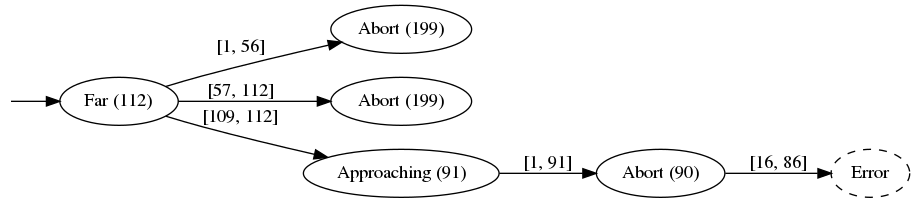
\includegraphics[width=0.9\textwidth]{images/viz2}
\caption{Example of an aggdag.}
\label{fig:aggdagex1}
\end{figure}
%\vspace{-0.5cm}

%\vspace{-0.3cm}
\begin{example}
Figure~\ref{fig:aggdagex1} is an example of aggdag where the hybrid automata has 3 modes of operation, namely, {\em Far}, {\em Approaching}, and {\em Abort}. The initial set starting from the Far mode takes the discrete transitions to Abort in the time duration $[1,56]$ and $[57,112]$ and stays in the Abort mode without encountering any unsafe set. The successors of the stars that encounter a discrete transition to the Approaching mode in the time interval $[109,112]$, encounter the unsafe set in future. In the Figure~\ref{fig:aggdagex1}, the star representing the node Approaching is the collection of the stars that encounter the discrete transition in the time interval $[109, 112]$. Simiarly, the node Abort [Abort (90) to be more precise] corresponds to the collection of the stars that take the discrete transition from Approaching mode to the Abort mode. Out of the stars in the Abort(90) node, the violation of safety propery happens between the time intervals $[16,86]$.
\end{example}

To check if the safety property is indeed violated in the reachable set computation, we first inspect the aggdag in Figure~\ref{fig:aggdagex1}. Since the safety is violated in trajectories in Abort mode, we need to inspect whether there is overapproximation induced in the aggregation of the reachable set in the path from the root node to the Abort node. 
This overapproximation can be at two instances, first, the aggregation of stars in the Approaching modes in the interval $[109, 112]$ or second, in the Abort mode in the interval $[1,91]$.  If both these reachable set do not have any aggregation, then we have proof that the overlap with the unsafe set is indeed a safety violation. Hence, refining only the aggregation associated with the reachable sets in the specific interval of time suffices.


The aggdag is useful only in bookkeeping the states that encounter the discrete transitions. The strategy for deaggregation is still decided by the user. In our tool, we have implemented two deaggregation strategies, first, from the leaf to root and second, from root to leaf. In the case of leaf to root, we first deaggregate the reachable sets that are closest to the safety violation and continue the deaggregation to the top. In Figure~\ref{fig:aggdagex1}, in the leaf to root strategy, we would first deaggregate the states taking the discrete transition from Approaching to Abort. In the root to leaf strategy, the deaggregation is performed at the node closest to the root node in the path leading to the unsafe overlap. In Figure~\ref{fig:aggdagex1}, under the root to leaf strategy, one would deaggregate the stars in the discrete transition from Far to Approaching. The best deaggregation strategy for proving safety or discovering the counterexample is still an area to be investigated and is a part of future research.






